% the name in brackets is the one used in the contents
\chapter[A chapter with long title]{A chapter with a very long \\ title that wouldn't fit}\label{ch:2-abm}
\markboth{Name of the chapter in the header}{}

This document uses Helvetica for the section and chapter titles, and Palatino for the text and equations (see \code{packages.tex}). Font size is set to 12pt, and line spacing to 1.2pt.



\section{The first section}


\subsection{The first subsection}

\begin{proposition}\label{prop:example}
    Definitions, propositions, and more theorem environments are defined in \code{macros.tex}.
    \begin{itemize}
        \item The default bullet point for \code{itemize} is changed to this one.
        \item Code is written using the command \code{\textbackslash code\{\}}.
    \end{itemize}
\end{proposition}

We can plot functions using \LaTeX, as shown in Figure \ref{fig:example-function}.

\begin{figure}[htp]
    \centering
    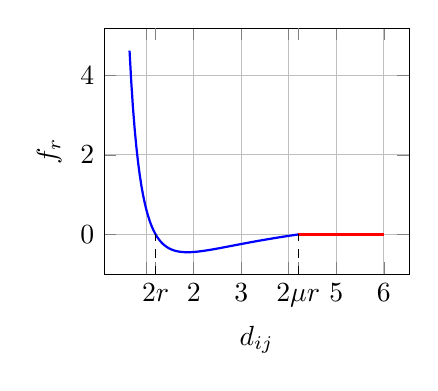
\begin{tikzpicture}
        \begin{axis}[
            width=0.45\textwidth,
            xlabel={$d_{ij}$}, 
            ylabel={$f_r$},
            % title={title}
            grid=both,
            domain=0:6,
            samples=100, 
            ymin=-1,
            xtick={1, 2, 3, 4, 5, 6},
            xticklabels={,2,3,,5,6}, 
            extra x ticks={1.2, 4.2}, 
            extra x tick labels={$2r$, $2\mu r$},
            extra x tick style={grid=none}
        ]
            \addplot[domain=0.65:4.2, samples=100, thick, color=blue] {(2*0.6/x - 1)*(2*.6*3.5/x - 1)};
            \addplot[domain=4.2:6, samples=100, thick, color=red] {0};

            \addplot[dashed, thin, black] coordinates {(1.2, -1) (1.2, 0)};
            \addplot[dashed, thin, black] coordinates {(4.2, -1) (4.2, 0)};
        \end{axis}
    \end{tikzpicture}    
    \caption{Example function $f_r$.}
    \label{fig:example-function}
\end{figure}

Recall that the example function $f_r$ is given by the following expression,
\begin{equation}\label{eq:example-function}
    f_r=
    \begin{dcases}
        \frac{a}{b}\alpha_\text{sub} &\quad \text{if $a<c$} \\
        ab\sqrt{a+c} &\quad \text{if $a\geq c$} \\
        0 &\quad \text{otherwise.}
    \end{dcases}
\end{equation}


\subsection{The second subsection}

Nesting in \code{enumerate}:

\begin{enumerate}
    \item First.
    \begin{enumerate}[label=\roman*.] % [label=\theenumi.\arabic*.]
        \item First first.
        \item Second first.
    \end{enumerate}
    \item Second.
\end{enumerate}

We can recall an equation while keeping the numbering. If there is a space between the text and the text and the \code{equation} environment, the space between these will increase because the equation will be assumed to be a separate paragraph. Keep this in mind to ensure consistency.
\begin{equation}\tag{\ref{eq:example-function}}
    f_r=
    \begin{dcases}
        \frac{a}{b}\alpha_\text{sub} &\quad \text{if $a<c$} \\
        ab\sqrt{a+c} &\quad \text{if $a\geq c$} \\
        0 &\quad \text{otherwise.}
    \end{dcases}
\end{equation}

If there is a space between the text and the text and the \code{equation} environment, the space between these will increase because the equation will be assumed to be a separate paragraph. Keep this in mind to ensure consistency.

\begin{equation}\tag{\ref{eq:example-function}}
    f_r=
    \begin{dcases}
        \frac{a}{b}\alpha_\text{sub} &\quad \text{if $a<c$} \\
        ab\sqrt{a+c} &\quad \text{if $a\geq c$} \\
        0 &\quad \text{otherwise.}
    \end{dcases}
\end{equation}

\begin{redbox}
    This is a custom environment for red boxes.
\end{redbox}

We can also\todo{like this} use margin notes. \tocite{like this}